%%==================================================
%% diss.tex for SJTU Master Thesis
%% based on CASthesis
%% modified by wei.jianwen@gmail.com
%% version: 0.3a
%% Encoding: UTF-8
%% last update: Dec 5th, 2010
%%==================================================

% 字号选项: c5size 五号(默认) cs4size 小四
% 双面打印(注意字号设置)
\documentclass[cs4size, a4paper, twoside]{sjtuthesis} 
% 单面打印(注意字号设置)
% \documentclass[cs4size, a4paper, oneside, openany]{sjtuthesis} 


% \usepackage[sectionbib]{chapterbib}%每章都用参考文献

\newboolean{DOIT}
\setboolean{DOIT}{false}%编译某些只想自己看的内容,编译true,否则false

%% 行距缩放因子(x倍字号)
\renewcommand{\baselinestretch}{1.3}

% 设置图形文件的搜索路径
\graphicspath{{figure/}{figures/}{logo/}{logos/}{graph/}{graphs}}

%%========================================
%% 在sjtuthesis.cls中定义的有用命令
%%========================================
% \cndash 中文破折号
% 数学常量
% \me 对数常数e
% \mi 虚数单位i
% \mj 虚数单位j
% \dif 直立的微分算符d为直立体。
% 可伸长的数学箭头、等号
% \myRightarrow{}{}
% \myLeftarrow{}{}
% \myBioarrow{}{}
% \myLongEqual{}{}
% 参考文献
% \upcite{} 上标引用
%%========================================


\begin{document}

%%%%%%%%%%%%%%%%%%%%%%%%%%%%%% 
%% 封面
%%%%%%%%%%%%%%%%%%%%%%%%%%%%%% 

% 中文封面内容(关注内容而不是形式)
\title{上海交通大学硕士学位论文~\XeTeX/\LaTeX~模板~\version}
\author{李\quad{}四}
\advisor{张三教授}
\degree{硕士}
\defenddate{2010年1月16日}
\school{上海交通大学}
\institute{物理系}
\studentnumber{0010900990}
\major{专业名称}

% 英文封面内容(关注内容而不是表现形式)
\englishtitle{\XeTeX/\LaTeX\, Template for SJTU Master Degree Thesis \version}
\englishauthor{\textsc{Si Li}}
\englishadvisor{Prof. \textsc{San Zhang}}
\englishschool{Shanghai Jiao Tong University}
\englishinstitute{\textsc{Depart of XXX, School of XXX} \\
  \textsc{Shanghai Jiao Tong University} \\
  \textsc{Shanghai, P.R.China}}
\englishdegree{Master}
\englishmajor{Physics}
\englishdate{Jan. 16th, 2010}

% 封面
\maketitle

% 英文封面
\makeenglishtitle

% 论文原创性声明和使用授权
\makeDeclareOriginal
\makeDeclareAuthorization

%%%%%%%%%%%%%%%%%%%%%%%%%%%%%% 
%% 前言
%%%%%%%%%%%%%%%%%%%%%%%%%%%%%% 
\frontmatter

% 摘要
%%==================================================
%% abstract.tex for SJTU Master Thesis
%% based on CASthesis
%% modified by wei.jianwen@gmail.com
%% version: 0.3a
%% Encoding: UTF-8
%% last update: Dec 5th, 2010
%%==================================================

\begin{abstract}

  上海交通大学是我国历史最悠久的高等学府之一,是教育部直属、教育部与上海市共建的全国重点大学,是国家 “七五”、“八五”重点建设和“211工程”、“985工程”的首批建设高校。经过115年的不懈努力,上海交通大学已经成为一所“综合性、研究型、国际化”的国内一流、国际知名大学,并正在向世界一流大学稳步迈进。 

 十九世纪末,甲午战败,民族危难。中国近代著名实业家、教育家盛宣怀和一批有识之士秉持“自强首在储才,储才必先兴学”的信念,于1896年在上海创办了交通大学的前身——南洋公学。建校伊始,学校即坚持“求实学,务实业”的宗旨,以培养“第一等人才”为教育目标,精勤进取,笃行不倦,在二十世纪二三十年代已成为国内著名的高等学府,被誉为“东方MIT”。抗战时期,广大师生历尽艰难,移转租界,内迁重庆,坚持办学,不少学生投笔从戎,浴血沙场。解放前夕,广大师生积极投身民主革命,学校被誉为“民主堡垒”。

 新中国成立初期,为配合国家经济建设的需要,学校调整出相当一部分优势专业、师资设备,支持国内兄弟院校的发展。五十年代中期,学校又响应国家建设大西北的号召,根据国务院决定,部分迁往西安,分为交通大学上海部分和西安部分。1959年3月两部分同时被列为全国重点大学,7月经国务院批准分别独立建制,交通大学上海部分启用“上海交通大学”校名。历经西迁、两地办学、独立办学等变迁,为构建新中国的高等教育体系,促进社会主义建设做出了重要贡献。六七十年代,学校先后归属国防科工委和六机部领导,积极投身国防人才培养和国防科研,为“两弹一星”和国防现代化做出了巨大贡献。

   改革开放以来,学校以“敢为天下先”的精神,大胆推进改革:率先组成教授代表团访问美国,率先实行校内管理体制改革,率先接受海外友人巨资捐赠等,有力地推动了学校的教学科研改革。1984年,邓小平同志亲切接见了学校领导和师生代表,对学校的各项改革给予了充分肯定。在国家和上海市的大力支持下,学校以“上水平、创一流”为目标,以学科建设为龙头,先后恢复和兴建了理科、管理学科、生命学科、法学和人文学科等。1999年,上海农学院并入;2005年,与上海第二医科大学强强合并。至此,学校完成了综合性大学的学科布局。近年来,通过国家“985工程”和“211工程”的建设,学校高层次人才日渐汇聚,科研实力快速提升,实现了向研究型大学的转变。与此同时,学校通过与美国密西根大学等世界一流大学的合作办学,实施国际化战略取得重要突破。1985年开始闵行校区建设,历经20多年,已基本建设成设施完善,环境优美的现代化大学校园,并已完成了办学重心向闵行校区的转移。学校现有徐汇、闵行、法华、七宝和重庆南路(卢湾)5个校区,总占地面积4840亩。通过一系列的改革和建设,学校的各项办学指标大幅度上升,实现了跨越式发展,整体实力显著增强,为建设世界一流大学奠定了坚实的基础。

  交通大学始终把人才培养作为办学的根本任务。一百多年来,学校为国家和社会培养了20余万各类优秀人才,包括一批杰出的政治家、科学家、社会活动家、实业家、工程技术专家和医学专家,如江泽民、陆定一、丁关根、汪道涵、钱学森、吴文俊、徐光宪、张光斗、黄炎培、邵力子、李叔同、蔡锷、邹韬奋、陈敏章、王振义、陈竺等。在中国科学院、中国工程院院士中,有200余位交大校友;在国家23位“两弹一星”功臣中,有6位交大校友;在18位国家最高科学技术奖获得者中,有3位来自交大。交大创造了中国近现代发展史上的诸多“第一”:中国最早的内燃机、最早的电机、最早的中文打字机等;新中国第一艘万吨轮、第一艘核潜艇、第一艘气垫船、第一艘水翼艇、自主设计的第一代战斗机、第一枚运载火箭、第一颗人造卫星、第一例心脏二尖瓣分离术、第一例成功移植同种原位肝手术、第一例成功抢救大面积烧伤病人手术等,都凝聚着交大师生和校友的心血智慧。改革开放以来,一批年轻的校友已在世界各地、各行各业崭露头角。

 截至2011年12月31日,学校共有24个学院/直属系(另有继续教育学院、技术学院和国际教育学院),19个直属单位,12家附属医院,全日制本科生16802人、研究生24495人(其中博士研究生5059人);有专任教师2979名,其中教授835名;中国科学院院士15名,中国工程院院士20名,中组部“千人计划”49名,“长江学者”95名,国家杰出青年基金获得者80名,国家重点基础研究发展计划(973计划)首席科学家24名,国家重大科学研究计划首席科学家9名,国家基金委创新研究群体6个,教育部创新团队17个。

  学校现有本科专业68个,涵盖经济学、法学、文学、理学、工学、农学、医学、管理学和艺术等九个学科门类;拥有国家级教学及人才培养基地7个,国家级校外实践教育基地5个,国家级实验教学示范中心5个,上海市实验教学示范中心4个;有国家级教学团队8个,上海市教学团队15个;有国家级教学名师7人,上海市教学名师35人;有国家级精品课程46门,上海市精品课程117门;有国家级双语示范课程7门;2001、2005和2009年,作为第一完成单位,共获得国家级教学成果37项、上海市教学成果157项。

  \keywords{\large 上海交大 \quad 饮水思源 \quad 爱国荣校}
\end{abstract}

\begin{englishabstract}

An imperial edict issued in 1896 by Emperor Guangxu, established Nanyang Public School in Shanghai. The normal school, school of foreign studies, middle school and a high school were established. Sheng Xuanhuai, the person responsible for proposing the idea to the emperor, became the first president and is regarded as the founder of the university.

During the 1930s, the university gained a reputation of nurturing top engineers. After the foundation of People's Republic, some faculties were transferred to other universities. A significant amount of its faculty were sent in 1956, by the national government, to Xi'an to help build up Xi'an Jiao Tong University in western China. Afterwards, the school was officially renamed Shanghai Jiao Tong University.

Since the reform and opening up policy in China, SJTU has taken the lead in management reform of institutions for higher education, regaining its vigor and vitality with an unprecedented momentum of growth. SJTU includes five beautiful campuses, Xuhui, Minhang, Luwan Qibao, and Fahua, taking up an area of about 3,225,833 m2. A number of disciplines have been advancing towards the top echelon internationally, and a batch of burgeoning branches of learning have taken an important position domestically.

Today SJTU has 31 schools (departments), 63 undergraduate programs, 250 masters-degree programs, 203 Ph.D. programs, 28 post-doctorate programs, and 11 state key laboratories and national engineering research centers.

SJTU boasts a large number of famous scientists and professors, including 35 academics of the Academy of Sciences and Academy of Engineering, 95 accredited professors and chair professors of the "Cheung Kong Scholars Program" and more than 2,000 professors and associate professors.

Its total enrollment of students amounts to 35,929, of which 1,564 are international students. There are 16,802 undergraduates, and 17,563 masters and Ph.D. candidates. After more than a century of operation, Jiao Tong University has inherited the old tradition of "high starting points, solid foundation, strict requirements and extensive practice." Students from SJTU have won top prizes in various competitions, including ACM International Collegiate Programming Contest, International Mathematical Contest in Modeling and Electronics Design Contests. Famous alumni include Jiang Zemin, Lu Dingyi, Ding Guangen, Wang Daohan, Qian Xuesen, Wu Wenjun, Zou Taofen, Mao Yisheng, Cai Er, Huang Yanpei, Shao Lizi, Wang An and many more. More than 200 of the academics of the Chinese Academy of Sciences and Chinese Academy of Engineering are alumni of Jiao Tong University.

  \englishkeywords{\large SJTU, master thesis, XeTeX/LaTeX template}
\end{englishabstract}


% 目录
\tableofcontents
% 插图索引
\listoffigures
\addcontentsline{toc}{chapter}{\listfigurename} %将图索引加入全文目录
% 表格索引
\listoftables
\addcontentsline{toc}{chapter}{\listtablename}  %将表格索引加入全文目录

% 主要符号、缩略词对照表
%%==================================================
%% symbol.tex for SJTU Master Thesis
%% based on CASthesis
%% modified by wei.jianwen@gmail.com
%% version: 0.3a
%% Encoding: UTF-8
%% last update: Dec 5th, 2010
%%==================================================

\chapter{主要符号对照表}
\label{chap:symb}
\begin{tabular}{ll}

 \hspace{2em}$\epsilon$       & \hspace{5em}介电常数 \\
 \hspace{2em}$\mu$ \qquad     & \hspace{5em}磁导率 \\
  \hspace{2em}$\epsilon$       & \hspace{5em}介电常数 \\
 \hspace{2em}$\mu$ \qquad     & \hspace{5em}磁导率 \\
 \hspace{2em}$\epsilon$       & \hspace{5em}介电常数 \\
 \hspace{2em}$\mu$ \qquad     & \hspace{5em}磁导率 \\
 \hspace{2em}$\epsilon$       & \hspace{5em}介电常数 \\
 \hspace{2em}$\mu$ \qquad     & \hspace{5em}磁导率 \\


\end{tabular}


%%%%%%%%%%%%%%%%%%%%%%%%%%%%%% 
%% 正文
%%%%%%%%%%%%%%%%%%%%%%%%%%%%%% 
\mainmatter


%% 各章正文内容
%%==========================
%% chapter01.tex for SJTU Master Thesis
%% based on CASthesis
%% modified by wei.jianwen@gmail.com
%% version: 0.3a
%% Encoding: UTF-8
%% last update: Dec 5th, 2010
%%==================================================

%\bibliographystyle{sjtu2} %[此处用于每章都生产参考文献]
\chapter{这是什么}
\label{chap:what}

这是上海交通大学(非官方)硕士学位学位论文 \LaTeX 模板,当前版本是 \version 。

\section{模板的来历}

最早的一版交大学位论文 \LaTeX 模板是一位热心的物理系同学制作的。
那份模板参考了自动化所学位论文模板,使用了CASthesis.cls文档类,中文字符处理则采用当时最为流行的 \CJKLaTeX 方案。
我根据交大研究生院对学位论文的要求进行了调整,完成了一份基本可用的交大 \LaTeX 学位论文模板。

但是,搭建一个 \CJKLaTeX 环境并不简单,在Linux下配置环境和调用中文字体的流程,对我而言犹如梦魇一般。
在William Wang的建议下,我开始着手把模板移植到 \XeTeX 上。
他完成了最初的移植,谢谢他的出色工作,使得后续的工作比我预想中的顺利。

这个学位论文模板从我用它来完成学位学位论文以后,就没有更新过。
过了快两年,随着知识水平的提高,我又想断断续续再做一些完善模板的工作,因此对原有的硕士论文模板做了修改,并在此基础上做了交大学士和博士学位论文 \LaTeX 模板。

现在,交大学位论文 \LaTeX 模板的代码在github上维护,地址是:

	\url{https://github.com/weijianwen/sjtu-thesis-template-latex/}

学士学位论文、硕士学位论文、博士学位论文分别在bachelor-thesis,master-thesis和phd-thesis分支中维护。
从下面的链接中可分别获得做新交大学士、硕士、博士模板zip压缩包,当前版本为\version 。

\begin{itemize}
	\item \href{https://github.com/weijianwen/sjtu-thesis-template-latex/archive/bachelor-0.5.3.zip}{交大学士学位论文模板\version} 
	\item \href{https://github.com/weijianwen/sjtu-thesis-template-latex/archive/master-0.5.3.zip}{交大硕士学位论文模板\version}
	\item \href{https://github.com/weijianwen/sjtu-thesis-template-latex/archive/phd-0.5.3.zip}{交大博士学位论文模板\version}
\end{itemize}

欢迎大家使用交大学位论文模板!你可以通过如下的途径反馈模板使用过程中遇到的问题:\href{https://github.com/weijianwen/sjtu-thesis-template-latex/issues}{开issue}
、\href{https://bbs.sjtu.edu.cn/bbsdoc?board=TeX_LaTeX}{水源LaTeX版}发帖,或者是给\href{mailto:weijianwen@gmail.com}{我}发送邮件---你可能需要好几天才能收到我的邮件回复。

\section{模板说明}
\subsection{模板特性}
\label{sec:features}

这个模板使用的中文解决方案是 \XeTeX/\LaTeX 。
参考文献使用BibTeX处理,可以生成符合国标GBT7714风格的参考文献列表。
模板在Windows,Linux和Mac OS X下测试通过,更详细的系统要求请参考\ref{sec:requirements}。

模板的外观表现和功能都放在sjtuthesis.cls和sjtuthesis.cfg中,在对外观进行细微调整时,只需要更新这两个文件,不需要对.tex源文件做修改。

最后,给出一个列表,罗列一下这个模板的功能要点:

\begin{itemize}
\item 使用 \XeTeX 引擎处理中文;
\item 包含中文字符的源文件(.tex, .bib, .cfg),编码都使用UTF-8;
\item 使用BibTeX处理参考文献。参考文献表现形式(格式)受.bst控制,方便在不同风格间切换,目前生成的列表符合国标GBT7714要求;
\item 可以直接插入EPS/PDF/JPG/PNG格式的图像,并且\emph{不需要}bounding box文件(.bb)。
\item 模板的格式受sjtumater-xetex.cls和sjtuthesis.cfg控制,方便模板更新和模板修改。
\end{itemize}

\subsection{系统要求}
\label{sec:requirements}

要使用这个模板协助你完成研究生学位论文的创作,下面的条件必须满足:

\begin{itemize}
\item 操作系统字体目录中有TeX Gyre Termes西文的:Regular, Italic, Bold, Bold Italic四种OTF字体\footnote{TeX Gyre Termes字体可以从\href{http://www.gust.org.pl/projects/e-foundry/tex-gyre/termes}{http://www.gust.org.pl/projects/e-foundry/tex-gyre/termes}下载。我也附带了一份TeX.Gyre.Termes.Fonts.zip在模板中,解压缩到字体目录后用fc-cache -fv刷新即可,用fc-list应该能看到。};
\item 操作系统字体目录中有AdobeSongStd、AdobeKaitiStd、AdobeHeitiStd、AdobeFangsongStd四款中文字体\footnote{Adobe这四款中文OTF字体可以从Adobe Reader安装目录拿到。};
\item \TeX 系统有 \XeTeX 引擎;
\item \TeX 系统有ctex宏包;
\item 你有使用 \LaTeX 的经验。
\end{itemize}

你可以试着编译模板文件夹中自带的test.tex文件,看看你的 \TeX 系统是否满足上面的要求:

\begin{lstlisting}[basicstyle=\small\ttfamily, caption={编译测试文件test.tex}, numbers=none]
xelatex test.tex
\end{lstlisting}

如果编译出的test.pdf中能够:显示中英文内容、显示4幅图像、正确嵌入AdobeSongStd和TeXGyreTermes字体(通过PDF阅读器的“属性”查看)、并且看到了英文字符的连字(ligature)和\textsc{SmallCapital}特性,那么恭喜你,你的 \TeX 系统应该能够编译这个学位论文模板。

目前,我在手头的几个 \TeX 环境上都做过测试,MacTeX 2011, TeXLive 2011和C\TeX 2.9都能够顺利编译。在你到版上抱怨模板不能工作前,请确定你的 \TeX 系统能够编译前面的test.tex文件。欢迎大家到\href{https://bbs.sjtu.edu.cn/bbsdoc?board=TeX_LaTeX}{水源LaTeX版}反馈问题。为了提高解决问题的速度,请在帖子中说明:是否顺利编译模板、错误提示、操作系统版本、\TeX 系统版本和最近对 \TeX 系统做的操作(如升级等)。
 
\subsection{模板文件布局}
\label{sec:layout}

\begin{lstlisting}[basicstyle=\small\ttfamily,caption={模板文件布局},label=layout,float,numbers=none]
  |-- diss.tex
  |-- README.pdf
  |-- sjtuthesis.cfg
  |-- sjtuthesis.cls
  |-- body
  |   |-- abstract.tex
  |   |-- app1.tex
  |   |-- app2.tex
  |   |-- chapter01.tex
  |   |-- chapter02.tex
  |   |-- conclusion.tex
  |   |-- projects.tex
  |   |-- pub.tex
  |   |-- resume.tex
  |   |-- symbol.tex
  |   \-- thanks.tex
  |-- figures
  |   \-- chap2
  |-- GBT7714-2005NLang.bst
  |-- Makefile
  |-- reference
  |   |-- chap1.bib
  |   \-- chap2.bib
  |-- test.tex
  \-- test.pdf
\end{lstlisting}

你拿到手的模板文件大致会包含代码\ref{layout}所列的文件,乍看起来还是挺令人头大的。
并且,这还是“干净”的时候,等到真正开始处理的时候,会冒出相当多的“中间文件”,这又会使情况变得更糟糕。
所以,有必要对这些文件做一些简要说明。
看完这部分以后,你应该发现,其实你要关心的文件类型并没有那么多。

\subsubsection{格式控制文件}
\label{sec:format}

格式控制文件控制着论文的表现形式,包括以下几个文件:
sjtuthesis.cfg, sjtuthesis.cls和GBT7714-2005NLang.bst。
其中,``.cfg''和``.cls''控制论文主体格式,``.bst''控制参考文献条目的格式,

一般用户最好``忽略''格式控制文件的存在,不要去碰它们。
有其他格式需要,欢迎到板上发贴。
对于因为擅自更改格式控制文件出现的问题,我不一定能够解决。

\subsubsection{主控文件diss.tex}
\label{sec:disstex}

主控文件diss.tex的作用就是将你分散在多个文件中的内容``整合''成一篇完整的论文。
使用这个模板撰写学位论文时,你的学位论文内容和素材会被``拆散''到各个文件中:
譬如各章正文、各个附录、各章参考文献等等。
在diss.tex中通过``include''命令将论文的各个部分包含进来,从而形成一篇结构完成的论文。
封面页中的论文标题、作者等中英文信息,也是在diss.tex中填写。
部分可能会频繁修改的设置,譬如行间距、图片文件目录等,我也放在了diss.tex中。
你也可以在diss.tex中按照自己的需要引入一些的宏包
\footnote{我对宏包的态度是:只有当你需要在文档中使用那个宏包时,才需要在导言区中用usepackage引入该宏包。如若不然,通过usepackage引入一大堆不被用到的宏包,必然是一场灾难。由于一开始没有一致的设计目标,\LaTeX 的各宏包几乎都是独立发展起来的,因重定义命令导致的宏包冲突屡见不鲜。}
。

大致而言,在diss.tex中,大家只要留意把``章''一级的内容,以及各章参考文献内容包含进来就可以了。
需要注意,处理文档时所有的操作命令 \cndash{} xelatex, bibtex等,都是作用在diss.tex上,而\emph{不是}后面这些``分散''的文件,请参考\ref{sec:process}小节。

\subsubsection{论文主体文件夹body}
\label{sec:thesisbody}

这一部分是论文的主体,是以``章''为单位划分的。

正文前部分(frontmatter):中英文摘要(abstract.tex)。其他部分,诸如中英文封面、授权信息等,都是根据diss.tex所填的信息``画''好了,
不单独弄成文件。

正文部分(mainmatter):自然就是各章内容chapter\emph{xxx}.tex了。

正文后的部分(backmatter):附录(app\emph{xx}.tex);致谢(thuanks.tex);攻读学位论文期间发表的学术论文目录(pub.tex);个人简历(resume.tex)。
参考文献列表是``生成''的,也不作为一个单独的文件。另外,学校的硕士研究生学位论文模板中,也没有要求加入个人简历,所以我没有在diss.tex中引入resume.tex。

\subsubsection{图片文件夹figures}
\label{sec:figuresdir}

figures文件夹放置了需要插入文档中的图片文件(PNG/JPG/PDF/EPS),建议按章再划分子目录。

\subsubsection{参考文献数据库文件夹reference}
\label{sec:bibdir}

reference文件夹放置的是各章``可能''会被引用的参考文献文件。
参考文献的元数据,例如作者、文献名称、年限、出版地等,会以一定的格式记录在纯文本文件.bib中。
最终的参考文献列表是BibTeX处理.bib后得到的,名为diss.bbl。
将参考文献按章划分的一个好处是,可以在各章后生成独立的参考文献,不过,现在看来没有这个必要。
关于参考文献的管理,可以进一步参考第\ref{chap:example}章中的例子。

\subsection{如何使用模板}
\label{sec:process}

模板的 \LaTeX 源文件需要用 \XeTeX 编译产生PDF文件。
我在此给出三种命令行下的编译方式:逐行手工执行、使用脚本、使用latexmk,大家可以根据自己的喜好,选择\emph{其中一种}完成工作。

\subsubsection{逐行手工执行}

模板使用 \XeTeX 引擎提供的xelatex的命令处理,作用于“主控文档”diss.tex。并且,可以省略扩展名。
在命令提示符下逐行敲入如下命令完成编译。

\begin{lstlisting}[basicstyle=\small\ttfamily, caption={手动执行编译过程}, numbers=none]
xelatex -no-pdf --interaction=nonstopmode diss
bibtex diss 
xelatex -no-pdf --interaction=nonstopmode diss 
xelatex --interaction=nonstopmode diss 
\end{lstlisting}

运行bibtex的时候会提示一些错误,猜测是{{\sc Bib}\TeX}对UTF-8支持不充分,一般不影响最终结果。留意因为拼写错误导致的``找不到文献错误''即可。

基本处理流程就是这样,一些 \LaTeX 排版的小例子可以参考第二章。

\subsubsection{使用脚本}

为方便使用,我把上面几条命令放到了两个脚本文件中。
Linux用户可以使用run.sh脚本,Windows用户可以使用run.bat。

\subsubsection{使用GNU make编译}

模板自带了一个简单的Makefile,使用make可以方便地完成相应任务,如 pdf, view, clean, distclean等。

\begin{lstlisting}[basicstyle=\small\ttfamily, caption={使用GNU make编译}, numbers=none]
make && make view
\end{lstlisting}

\section{从 \CJKLaTeX 转向 \XeTeX}
\label{sec:whydvipdfm}

我习惯把v0.2a使用dvipdfmx编译的硕士学位论文模板称为``\CJKLaTeX 模板'',而这个使用 \XeTeX 引擎(xelatex程序)处理的模板则被称为``\XeTeX/\LaTeX 模板''。
从 \CJKLaTeX 模板迁移到 \XeTeX\LaTeX 模板的好处有下:
\begin{enumerate}
\item[\large\smiley] 搭建 \XeTeX 环境比搭建 \CJKLaTeX 环境更容易;
\item[\large\smiley] 更简单的字体控制;
\item[\large\smiley] 完美支持PDF/EPS/PNG/JPG图片,不需要``.bb''文件;
\item[\large\smiley] 支持OpenType字体的复杂字型变化功能(通常只有字母字体才有,学术文章也暂时用不上);
\end{enumerate}

当然,这也是有代价的。由于 \XeTeX 比较新,在我看来,使用 \XeTeX 模板所必须付出的代价是:

\begin{enumerate}
\item[\large\frownie] 必须把你“古老的” \TeX 系统更新为较新的版本。TeXLive 2012和CTeX 2.9.2能够编译这份模板,而更早的版本则无能为力。
\item[\large\frownie] 需要花一些时间把你在老模板上的工作迁移到新模板上。
\end{enumerate}

第一条就看你如何取舍了,新系统通常意味着更好的兼容性,值得升级。而转换模板也不是什么特别困难的事情,可以这样完成:

\begin{enumerate}
\item 备份你要转换的源文件,以防你的工作成果丢失;
\item 将你原来的``.tex''和``.bib''文件"另存为"UTF-8编码的文件。iconv、vim、emacs、UEdit等等工具都可以完成。WinEdt对文件编码识别功能很差(到了v6.0还是如此),不推荐作为字符编码转换工具;
\item 将diss.tex导言区中的内容替换为XeTeX模板diss.tex导言区的内容;
\item 将你对原先导言区的修改,小心翼翼地``合并''到新的导言区中;
\item 使用XeTeX模板中的GBT7714-2005NLang.bst替换原有的bst文件,新的bst文件只是将字符编码转换为UTF--8。
\item 删除bouding box文件``.bb'';
\item 使用本文\ref{sec:process}介绍的方法,重新编译文档;
\end{enumerate}

\section{硕士学位论文格式的一些说明}
\label{sec:thesisformat}

所有关于研究生学位论文模板的要求,我参考的都是下面这个教务处的网址
\href{http://www.gs.sjtu.edu.cn/policy/fileShow.ahtml?id=130}{《上海交通大学研究生学位论文格式的统一要求 》}。

可惜,这个网址没有给出具体可用的“模板文件”。
并且,``要求''中的一些要求也不仅合理,譬如,公式和公式编号之前要用……连接,实现起来困难,看起来也不美观,从来没有人这样用,所以无视之。
师兄师姐的学位论文也是我可以参考的“范本”,尽管这些范本也不是很规范。
我希望制作出的这个学位论文模板尽可能符合教务处的要求,如果有任何建议,欢迎提出!

这个模板是为``双面打印''准备的,也就是说,迎面页总是奇数页,新的一章将从奇数页开始,``迎面页''和``背面页''(或者说奇数页和偶数页)的左右页眉是相互颠倒的,奇数页和偶数页的左右页边距也会被颠倒。通过双面打印得到的学位论文就像一本正常的书。

你可以将diss.tex中设定文档类的语句改为:

\begin{quote}
  {\scriptsize\verb+\documentclass[cs4size, a4paer, cs4size, oneside, openany]{sjtuthesis}+}
\end{quote}

这样,就变成了适合“单面打印”的论文,新的一章可以从偶数页开始。

关于页眉页脚。奇数页页眉为:左边``上海交通大学硕士学位论文'',右边:``章节名'';偶数页页眉为:左边``上海交通大学硕士学位论文'',右边:``论文题目''。每一章的内容按照排书的习惯,均从奇数页开始。

教务处要求参考文献必须符合GBT7714风格,学校明确提出使用这个标准而不是自己拍脑袋想出别的做法,应该算是谢天谢地了。使用这个模板,结合BibTeX,可以很方便地生成符合GB标准的参考文献列表。

\section{模板更新说明}
\label{sec:update}

我希望这个模板能够成为大家完成学位论文的助手。
我会在一段时间内(一个月?一年?),继续维护这个模板,修正其中的错误和不理想的地方。
我还计划向模板中添加常用的``例子'',譬如表格、公式、图片的排版,这也是我知识汇总的。
完整的更新记录可参考附录A.

不管怎么说,模板更新应该是一件好事。
如果``新的格式控制文件''产生的效果对你很有吸引力,那么不妨尝试一下。
应用新的格式控制文件是一件非常简单的事情:
你只要把原来的sjtuthesis.cls, sjtuthesis.cfg, GBxxx.bst覆盖(建议备份或者使用版本控制系统),重新编译一遍,应该就OK了。

我大力推荐大家使用\href{http://git-scm.com}{git}\cndash{}一个优秀的代码控制系统\cndash{}管理整个学位论文的协作过程。使用git合并(merge)最新版本的模板,是一件非常安全且无痛的工作。



%%==================================================
%% chapter02.tex for SJTU Master Thesis
%% based on CASthesis
%% modified by wei.jianwen@gmail.com
%% Encoding: UTF-8
%%==================================================

\chapter{背景介绍}
\label{chap:background}

本章简要描述了x86架构上系统虚拟化技术的演化历程,并对后文Secure KVM系统和FlexCore系统中涉及到的x86硬件辅助虚拟化技术进行了详细介绍。

\section{x86系统虚拟化技术的演化}

系统虚拟化毫无疑问是推动当前火热云计算大潮的关键技术之一。随着x86处理器凭借着高速增长的处理能力和相对低廉的价格逐渐获得市场的广泛认可,x86平台上的系统虚拟化技术在近20年内取得了长足发展,学术界和工业界中都涌现出了一批富有影响力的系统虚拟化产品,如Bochs\cite{lawton1996bochs}、Qemu\cite{bellard2005qemu}、Xen\cite{barham2003xen}、VMware\cite{sugerman2001virtualizing}、KVM\cite{kivity2007kvm}等。

系统虚拟化是一种资源管理技术,其对真实计算机上的处理器资源、内存资源、存储资源等进行分割并赋予虚拟机,让这些用软件实现抽象出来的虚拟机可以像真实机器一样运行程序。然而,x86处理器的设计初衷并没有囊括系统虚拟化在内,当时在大型主机上普遍适用的``陷入并模拟''(Trap-and-Emulate)虚拟化策略在x86体系结构上未能奏效\cite{robin2000analysis}。这是因为如果按照``陷入并模拟''策略让x86虚拟机以较低权限级别运行,某些敏感x86指令会默默地执行失败而不会产生到虚拟机监控器的陷入,即为虚拟化漏洞,例如POPF指令在Ring 3权限级别执行时不会对\%EFLAGS寄存器系统状态位产生影响也不会触发处理器异常,这便让虚拟机监控器失去了模拟这些敏感指令行为的机会。而Intel出于x86平台的向后兼容性考虑,不可能去改变已发布x86指令集的行为,这个困境在很长一段时间里阻碍了x86平台系统虚拟化的发展。

虽然存在不小的困境,但x86平台上的系统虚拟化还不至于无路可循。一种简单粗暴的解决方法便是``模拟执行''。具体而言,便是分配一个足够大的数组当做虚拟机的内存,根据x86指令集规范,编写一个包含众多case分支的switch语句,获取当前要执行的指令,严格遵照指令集规范说明模拟执行。以上``模拟执行''的方法固然可行,但效率不敢恭维,这种虚拟机至少要比真实机器慢上一个数量级,造成其应用范围非常有限。此外,所谓的动态类型语言,如Python、PHP、Ruby,在被编译成中间代码后,大多也是遵循了这种``模拟执行''的方法,因此执行速度相比于编译型语言快不起来。著名的x86模拟器Bochs便是采用了这种``模拟执行''方法,虽然速度慢,但是兼容性良好,而且不容易出现安全漏洞。

除了``模拟执行'',二进制翻译技术也能用于解决x86平台上的系统虚拟化困境,且具备性能上的优势。如今Java、.NET、JavaScript等语言使用的JIT(Just-In-Time)技术也都属于类似的套路。不能因为指令翻译难实现就因噎废食,一个运行上亿次的for循环,其中如果都是加减之类的数学运算操作,翻译成机器码在处理器上直接执行,肯定比``模拟执行''要快得多。应用到系统虚拟化领域时,在二进制翻译前面,要加上``动态''两字,也就是在虚拟机执行过程中,碰到能翻译的普通指令区块就翻译成目标架构的机器码直接执行,并缓存起来以便后续重复执行,碰到不能直接翻译的特殊指令区块(某些关乎处理器全局状态的敏感指令,例如更改页表地址寄存器值的MOV \%CR3指令)就陷入到虚拟机监控器中或调用虚拟机监控器提供的接口,让虚拟机监控器模拟执行敏感指令,接着再继续对后面的虚拟机代码进行翻译。

VMware的工程师们在1998年首先实现了基于动态二进制翻译(Dynamic Binary Translation)的虚拟机监控器,成功在x86平台上高效实现了系统虚拟化,并推出了VMware Workstation、VMware ESX等商业化产品\cite{agesen2010evolution}。Fabrice Bellard完成的Qemu实现原理与上述类似,不过Qemu还支持在x86平台上模拟ARM、MIPS、SPARC、PowerPC等多种处理器架构。VMware针对动态二进制翻译还额外提出了众多其他功能和细节上的优化,这使得其商业化产品性能良好。VMware在x86系统虚拟化领域的创举,也复苏了研究人员和硬件厂商重新发掘这个领域的热情。

动态二进制翻译虽然已经比``模拟执行''快了许多,但由于为了让每条敏感指令得到模拟执行,执行流都要往虚拟机监控器绕一圈(而事实上在大多数情况下,虚拟机内执行多条敏感指令仅仅是为了完成某个单一目的,如在使用了PAE分页机制的32位操作系统中修改某一页表项需要两条MOV指令),这使得虚拟机离真实机器的性能仍然有一定差距。为了提升虚拟机的运行性能,研究人员想到了让虚拟机操作系统辅助配合,即为所谓的``半虚拟化''(Para-virtualization)。``Para''前缀是``with''、``alongside''的意思,也就是说虚拟机与虚拟机监控器不再是严格的上下级关系,而是互信合作的关系。虚拟机操作系统知道自己正处在虚拟化层之上运行,虚拟化层也要在一定程度上信任虚拟机操作系统。Xen在初始阶段便是一个只支持半虚拟化的虚拟化平台,但它为x86系统虚拟化领域开启了新的篇章。

既然动态二进制翻译的难点和性能瓶颈在于模拟执行那些各式各样的敏感指令,我们能不能修改虚拟机的操作系统内核,把那些敏感指令改得``好看''一些,即对虚拟化更友好?以上便是半虚拟化技术的核心思想。毕竟在大多数情况下,我们并不需要对虚拟机刻意``隐瞒'' 虚拟化层的存在,而是要在虚拟机之间提供必要的隔离,同时又不至于造成太多的性能开销。

采用半虚拟化的虚拟机操作系统内核需要经过特殊修改,将原先由敏感指令构成的操作改为对虚拟化层功能接口的调用,即超调用(Hypercall)。在现代操作系统中,由于这些特定体系结构相关的敏感操作实现都被封装起来了(例如Linux内核源码树中的arch/目录),对比动态二进制翻译需要考虑到各种边界情况,半虚拟化对虚拟机操作系统内核源码的修改就显得要简单一些了。相比于使用了动态二进制翻译的全虚拟化(Full-virtualization),半虚拟化是牺牲了通用性来换取性能,因为任何操作系统都可以无修改地运行在全虚拟化平台上,而每个半虚拟化的操作系统内核都要经过人工仔细修改,且要以能获取其源码为前提\cite{barham2003xen}\cite{bugnion1997disco}。

同样的功能,依靠专用硬件实现几乎总是比软件实现性能更好,这几乎已经成为了一条金科玉律。为了顺应市场对于高性能x86系统虚拟化的强烈愿求,Intel和AMD在2005年末几乎于相同的时间推出了x86硬件辅助虚拟化(Hardware-assisted Virtualization)解决方案,并在之后的发展历程中不断对其进行了增强。Intel的解决方案叫做Intel VT(Intel Virtualization Technology)或VMX(Virtual Machine Extension),AMD的解决方案被称为SVM(Secure Virtual Machine)。

在硬件上帮助软件系统实现以前难以完美解决的方案并不是一个新概念。早在1974年,Popek和Goldberg便在``Formal requirements for virtualizable third generation architectures''著名论文中提及了可虚拟化体系结构必须满足的三个必要条件\cite{popek1974formal}:1)虚拟机监控器提供与真实机器一模一样的虚拟环境;2)运行在虚拟机里的程序在最坏情况下也比物理机慢得不多;3)虚拟机监控器能够完全控制所有的系统资源;3a)虚拟机里的程序不能访问未分配给它的资源,3b)在某些情况下,虚拟机监控器能够回收已经分配给虚拟机的资源。早期的x86指令架构不满足上述条件,因而需要虚拟机监控器进行复杂的动态二进制翻译。既然动态二进制翻译的主要工作在于捕获虚拟机执行中的敏感指令,硬件辅助虚拟化中处理器最重要的职责便是捕获这些关键事件并将其交由虚拟机监控器处理。

为了维持对早期x86程序的兼容性,硬件辅助虚拟化在x86体系结构原有的四个执行特权级(Ring)基础上,增加了一个专供虚拟机监控器使用的与原先特权级别正交的根模式(Root mode),而虚拟机中的操作系统和应用程序则处于独立的非根模式(Non-root mode)运行。这样一来,尽管虚拟机操作系统运行在Ring 0,其执行敏感指令时仍然会触发异常并被处理器自动捕获,从而陷入到位于根模式的虚拟机监控器中,待到虚拟机监控器完成处理后再使用VMLAUNCH或VMRESUME指令让执行流返回虚拟机。

下一节将对硬件辅助虚拟化技术进行详细阐述。

\section{硬件辅助虚拟化技术}

\subsection{概述}

硬件辅助虚拟化技术,顾名思义,就是在处理器、芯片组和I/O设备等硬件层面上加入专门针对虚拟化的支持,让虚拟机监控器能够更容易、更高效率地实现系统虚拟化。

之所以要在硬件层面给予辅助,原因来自多方面。首先,由于原先x86体系结构存在虚拟化漏洞,单纯的``陷入并模拟''方案是行不通的,而动态二进制翻译技术难以处理虚拟机内的自修改代码和自参考代码,采用半虚拟化技术的前提是能够获取虚拟机内操作系统的源码;其次,由于硬件特性的限制,某些虚拟化功能尽管理论上可以用软件方法实现,但是实现途径异常曲折复杂,一个典型的例子便是限制虚拟机访存的影子页表(Shadow Page Table,SPT),其受限于原先处理器硬件只能提供一层内存地址转化功能;最后,某些使用软件方法实现的虚拟化功能往往性能和隔离性达不到要求,例如网卡磁盘等I/O设备的虚拟化。以上提及的这些问题,只有在处理器、芯片组等硬件层面上提供相应的辅助支持,才能得以完全解决。

两大处理器厂商Intel和AMD都想方设法要在系统虚拟化领域中占得先机,但是AMD的虚拟化技术在推出时间上要比Intel落后几个月。Intel自2005年末便开始在其处理器产品线中推广应用Intel VT(Intel Virtualization Technology)硬件辅助虚拟化技术。

AMD处理器提供的硬件辅助虚拟化技术虽然与Intel VT在细节上存在差异,不过它们的主体架构和核心思想是类似的,下文章节将以Intel VT为例详细介绍硬件辅助虚拟化技术。

\subsection{CPU虚拟化}

Intel VT在x86处理器原有的四个运行权限级别基础上,引入了两种新的操作模式,统称为VMX操作模式。

\begin{itemize}
\item VMX根模式(VMX Root Mode):虚拟机监控器所处的运行模式,基本等同于加入硬件辅助虚拟化支持以前的处理器工作模式,以下简称根模式。
\item VMX非根模式(VMX Non-Root Mode):客户虚拟机所处的运行模式,虚拟机内的二进制代码无需经过特殊处理以该模式在处理器硬件上直接运行,以下简称非根模式。
\end{itemize}

这两种VMX操作模式与32位x86处理器原有的Ring 0$\sim$Ring 3权限级别是正交的,即在每种VMX操作模式下都有Ring 0$\sim$Ring 3这四个运行权限级别。Intel VT采用这种改动方式的理由很明显,x86体系结构不能借助``陷入并模拟''这种经典方式进行系统虚拟化的根本原因在于其中的19条指令无法在低权限级别产生陷入,从而导致了虚拟化漏洞。如果简单地修改这19条指令的语义,让其在低权限级别运行时也能产生陷入,便会破坏与之前软件代码的二进制兼容性,而这是不可接受的。通过引入新的处理器运行模式,并重新定义敏感指令(包括之前的19条指令)在非根模式下的运行行为,即让其在非根模式运行时也能够产生到根模式的陷入,便能很好地填补先前的虚拟化漏洞。同时,Intel VT保持了x86原先所有指令在根模式下的运行语义不变,因此之前的二进制代码仍能正常运行。Intel VT通过这种途径很好地解决了x86系统虚拟化问题。

虚拟机在支持Intel VT技术的x86处理器上运行过程如图\ref{fig:mode}所示:

\begin{figure}[!htbp]
  \centering
  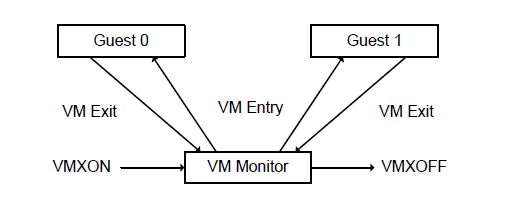
\includegraphics[width=0.7\textwidth]{chap2/mode.png}
  \bicaption[fig:mode]{Intel VT支持下的虚拟机的运行循环}{Intel VT支持下的虚拟机的运行循环}{Fig}{Virtual Machine Life Cycle with Intel VT}
\end{figure}

\begin{enumerate}
\item 虚拟机监控器执行VMXON指令让处理器进入VMX根模式,为运行客户虚拟机做准备。
\item 虚拟机监控器执行VMLAUNCH或者VMRESUME指令产生VM Entry,执行流转移至虚拟机内部的代码,处理器处于VMX非根模式运行。
\item 由于客户虚拟机执行了敏感指令,或者在其运行期间发生了硬件中断或软件异常,VM Exit被触发,执行流重新回到虚拟机监控器,处理器回到VMX根模式运行。
\item 虚拟机监控器根据虚拟化陷入发生的原因进行相应的处理,处理完成后,虚拟机监控器可以选择继续回到先前运行的客户虚拟机或者重新挑选另一个客户虚拟机运行,即回到步骤2。
\item 所有的客户虚拟机运行完毕,虚拟机监控器使用VMXOFF指令让处理器从VMX根模式退出。
\end{enumerate}

可以看出,虚拟机的顺利运行,就是一个在虚拟机监控器->虚拟机->虚拟机监控器->虚拟机->$\cdots\cdots$间不断循环的过程。以上流程中包含了两个处理器在VMX根模式和VMX非根模式间切换的行为,分别为从根模式切换到非根模式的VM Entry和从非根模式切换到根模式的VM Exit。

\begin{itemize}
\item VM Entry:虚拟机监控器在VMCS中设置好虚拟机接下来运行的上下文环境,使用VMLAUNCH(用于第一次或刚执行VMCLEAR后的VM Entry)或VMRESUME(用于执行过VMLAUNCH虚拟机的后续VM Entry)使处理器由根模式向非根模式转换,转换完成后,虚拟机内部的代码开始在处理器上直接执行。
\item VM Exit:由于某些原因,如虚拟机执行了敏感指令或发生了外部中断,处理器暂停执行虚拟机内部代码,从非根模式回退至根模式。虚拟机监控器会根据VM Exit发生的具体原因,对应地给予处理,如模拟指令行为等。在硬件辅助虚拟化中,处理VM Exit是虚拟机监控器最主要的职责。
\end{itemize}

VMCS(Virtual Machine Control Structure)被用于在虚拟机监控器和处理器硬件之间共享虚拟机执行的上下文环境和交换数据信息。虚拟机监控器可以通过修改VMCS中的某些位域来控制虚拟机在非根模式下的运行行为,在VM Exit发生时虚拟机监控器可以从VMCS中获取陷入发生的具体原因,此外虚拟机和宿主机某些关键寄存器的值在VM Exit和VM Entry发生时会在VMCS中进行保存和恢复。VMCS占用一个对齐的4KB大小的内存区域,即一个普通内存页框,其中主要的结构组成如下:

\begin{enumerate}
\item 客户虚拟机状态域,包括虚拟机部分关键寄存器的值、虚拟处理器可中断状态。
\item 宿主机状态域,主要是宿主机部分关键寄存器的值。
\item 虚拟机执行控制域,控制客户虚拟机在非根模式下的执行行为。
\item 虚拟化陷入控制域,控制虚拟化陷入的产生条件。
\item 虚拟机进入控制域,控制处理器从根模式向非根模式转换。
\item 虚拟化陷入信息域,记录了虚拟化陷入发生的具体原因,其值由硬件自动更新。
\end{enumerate}

Intel为了在处理器上支持硬件辅助虚拟化,扩展了原有的x86指令集,增添了13条新指令,列举如下。其中,除去VMCALL和VMFUNC被用于虚拟机内部在非根模式下执行,其余的11条指令适用于在处理器根模式下执行。

\begin{enumerate}
\item INVEPT:使EPT TLB中的特定内存地址翻译失效。
\item INVVPID:使与VPID对应的某虚拟机所有的内存地址翻译失效。
\item VMCALL/VMFUNC:发起向虚拟机监控器的请求调用。
\item VMCLEAR:将VMCS数据强制由处理器刷新回内存。
\item VMLAUNCH/VMRESUME:启动或唤醒虚拟机。
\item VMPTRLD/VMPTRST:加载或存储指向VMCS的内存地址。
\item VMREAD/VMWRITE:读取或写入当前加载VMCS的某些位域。
\item VMXON/VMXOFF:使处理器进入或离开VMX操作模式。
\end{enumerate}

\subsection{内存虚拟化}

在虚拟化环境中,存在着两层内存地址转换关系,即从客户虚拟机虚拟地址到客户虚拟机物理地址的第一层转换,和从客户虚拟机物理地址到宿主机物理地址的第二层转换。而在原先的x86处理器上,硬件只提供一层地址转换,即通过\%CR3控制寄存器指向的页表实现虚拟地址到物理地址的转换。因此,在以动态二进制翻译等技术软件实现的虚拟化平台上,虚拟机监控器需要为虚拟机内部的每一份页表对应维护一份影子页表(对于Linux,虚拟机监控器要为其中的每个进程维护一份影子页表,并在虚拟机内部发生进程切换时对应切换影子页表),此维护过程需要监视虚拟机内部对于页表的修改且要仔细处理可能发生的各种边界情况,增大了虚拟机监控器的设计实现难度,且会对虚拟机性能造成较大影响。

Intel在其2007推出的第二代硬件辅助虚拟化技术中增添了对于扩展页表(Extended Page Table,EPT)特性的支持\cite{adams2006comparison},直接在处理器硬件上支持两层内存地址转换,大大降低了内存虚拟化的实现难度,同时也提升了虚拟机的运行性能。

EPT表的大致结构与普通x86页表类似,两者都采用多级结构,其中每个EPT页表项的高位部分用于记录页框号,低12位则用于记录一些标志位(是否可读、是否可写、是否可执行、是否是超页)。VMCS中有专门的位域用于设置EPT表,虚拟机中代码的访存范围受到EPT表的限制。

\begin{figure}[!htbp]
  \centering
  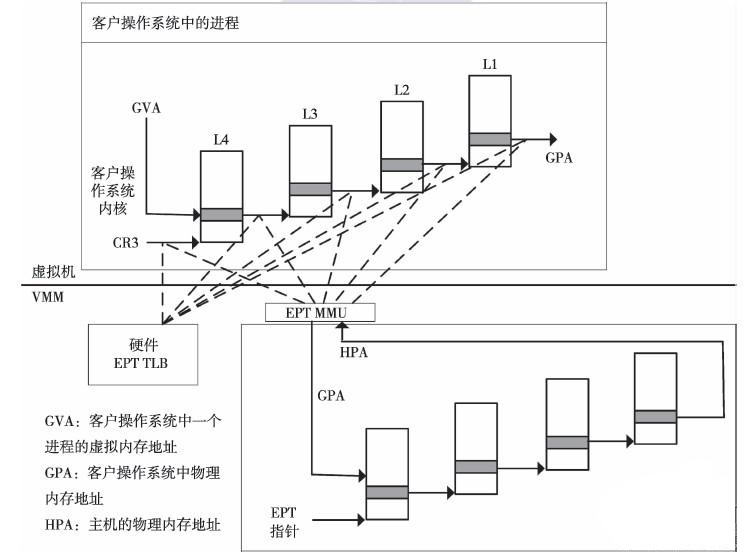
\includegraphics[width=0.7\textwidth]{chap2/ept.png}
  \bicaption[fig:ept]{EPT表内存地址翻译示意}{EPT表内存地址翻译示意}{Fig}{Illustration on Memory Address Translation of EPT}
\end{figure}

此处假设客户虚拟机中的普通页表和EPT表都是4级结构,处理器完成一次完整内存地址转换的流程如下。处理器首先根据虚拟机内\%CR3寄存器值获得L4页表地址,此L4页表地址为客户虚拟机物理地址(Guest Physical Address,GPA),因此处理器还要参考EPT表来实现该GPA到宿主机物理地址(Host Physical Address,HPA)的转换。处理器会先到TLB中进行查找,如果其中没有对应的缓存项,处理器再退而求其次到EPT表中逐级进行查找,如果仍没有找到,处理器则会抛出EPT页故障并交由虚拟机监控器处理。在获得L4页表的HPA后,处理器根据待翻译地址偏移和L4页表内容,来确定L3页表的GPA,之后再通过查找EPT表获取L3页表的HPA。按照类似的步骤,处理器依次访问L2和L1页表,获得待翻译地址对应的GPA,最后再通过EPT表转换为HPA,并将该映射关系在TLB中缓存。在以上内存地址翻译流程中,若是处于最不利情况即TLB为空时,处理器需要经历共计24(5*4+4)次访存,不过在之后TLB缓存生效情况下,虚拟机内的访存速度与非虚拟化环境下无异。为了提升虚拟机内的访存效率,处理器通过增大EPT TLB容量来减少地址翻译过程中的TLB缺失率。

\subsection{中断虚拟化}

虚拟机的运行离不开众多的I/O设备,例如磁盘和网卡,这些I/O设备一般都是由虚拟机监控器或专门的用户态程序如Qemu来进行模拟,而这些I/O设备的模拟离不开中断虚拟化。

在虚拟化环境中,虚拟机监控器为客户虚拟机维护了一套与真实物理机器上中断架构类似的虚拟中断架构,其中包括了虚拟PIC、虚拟Local APIC、虚拟I/O APIC等软件实体。当虚拟设备需要发送中断时,虚拟设备会调用虚拟I/O APIC提供的接口发送中断。虚拟I/O APIC根据中断具体情况,将中断路由至对应的虚拟Local APIC。虚拟Local APIC再进一步调用Intel VT中的事件注入机制将中断注入到对应的虚拟处理器。

\section{本章小结}

本章对论文中所涉及到的一些相关背景知识进行了介绍。本章在一开始先简要叙述了x86体系结构上系统虚拟化的发展历程,然后从CPU虚拟化、内存虚拟化和中断虚拟化三个方面着重介绍了x86上的硬件辅助虚拟化技术,为以后的章节做了铺垫。
%%==================================================
%% chapter03.tex for SJTU Master Thesis
%% Encoding: UTF-8
%%==================================================

\chapter{Secure KVM安全嵌套式虚拟化系统的设计与实现}
\label{chap:securekvm}



\section{引言}

\section{背景介绍及问题分析}

\subsection{虚拟化本质论}

所谓“系统虚拟化”,亦即VMM虚拟机监控器给客户操作系统和应用程序提供一个虚拟的运行平台,而这个虚拟运行平台要与真实硬件基本无异,不能让客户操作系统和应用程序感受到差别(现阶段,打通VMM虚拟机监控器和Guest VM客户虚拟机之间的语义隔阂,主动让客户虚拟机意识到自己运行在虚拟化平台上以获得性能提升的情形也是存在的,在本文中我们忽略这样的特例)。

对于一个虚拟的运行平台而言,有三个主要组成要素,分别是CPU、内存和外设(磁盘和网卡属于此类)。关于CPU,虚拟机监控器要将物理机器上的计算资源即CPU时间片分一部分给客户虚拟机,同时又必须保证CPU资源不能被某一客户虚拟机长期无节制地占用,以免耽误虚拟机监控器自身和其他客户虚拟机的正常运行(类似于操作系统和应用程序之间的关系)。对于内存,虚拟机监控器同样要在满足客户虚拟机内存资源分配的同时保证安全,即某一客户虚拟机必须有节制地使用内存,该客户虚拟机和虚拟机监控器、该客户虚拟机和其他客户虚拟机之间必须保证内存隔离。对于外设,虚拟机监控器要对他们的IO行为进行精确模拟,这一般是通过截获IO指令和MMIO读写操作来完成。

这所有的一些,均要求虚拟机监控器处在比客户虚拟机更高的运行级别。对于CPU,虚拟机监控器要在某一客户虚拟机时间片用完时(时间中断到来),立即获得执行机会抢占该客户虚拟机,并切换另一客户虚拟机上来运行。对于内存,虚拟机监控器要通过一些类似页表的硬件机制限制客户虚拟机的访存范围。对于截获IO指令和MMIO读写,这同样需要高运行级别和硬件机制来保证。

具体到x86硬件虚拟化,虚拟机监控器处在高权限级别的根模式(root mode),客户虚拟机处在低权限级别的非根模式(non-root mode)。当客户虚拟机处在非根模式运行期间发生时间中断时,处理器会以外部中断(External Interrupt)到来的原因陷入到根模式,让虚拟机监控器处理。2007之后Intel推出的第二代硬件虚拟化处理器,均支持扩展页表(Extended Page Table,简称EPT),可以在硬件层面上限制客户虚拟机的内存访问。最后,虚拟机监控器可以指定IO位图,让非根模式下期望的IO指令发生陷入(MMIO读写与此基本类似),并对其进行指令模拟以达到模拟真实设备行为的目的。

不可否认,为了达到系统虚拟化的目的,在一般情况下让虚拟机监控器处在高权限级别是一个必要条件。但与此同时带来的是,虚拟机监控器不受管控的“为所欲为”,给客户虚拟机运行的安全性和隐私性带来了重大隐患。此情形在多租户云、第三方虚拟机提供商等应用环境下体现得尤为明显。下面两节分别从内存和磁盘的角度对此进行详细阐述。

\subsection{客户虚拟机的内存安全}

客户虚拟机的内存中包含有其正在运行程序的所有信息,包括操作系统层面的进程信息、模块信息和应用程序地址空间中的所有数据、代码区域。举例来说,客户虚拟机中的浏览器打开了网银的登录界面而用户正在输入其账号密码,这些隐私数据都是会被保存到客户虚拟机的内存中。

扩展页表限制的是客户虚拟机的访存范围,而虚拟机监控器处在最高权限级别,其可以将物理上的任意内存区块映射到自己的地址空间,并进行访问改写。同样以上文用户网银登陆为例,恶意虚拟机监控器在得知这一信息后,可以对整个客户虚拟机的内存空间进行转储(dump),并在事后进行查找分析,导致用户的敏感隐私数据极有可能因此而被暴露偷窥。

尽管恶意虚拟机监控器起先获取的可能只是庞杂的原始字节数据,其可以利用特殊寄存器数据、特定操作系统内存地址空间结构等信息作为提示,借助虚拟机自省(Virtual Machine Introspection,VMI)等技术手段,从中萃取出隐私数据和语义信息,毕竟这在理论上是可能的。

\subsection{客户虚拟机的磁盘安全}

在真实机器上读磁盘的过程可以简化为此,操作系统先在内存中预留一段区域,然后将待读取数据在磁盘上的位置和预留内存地址等信息通过IO指令告诉磁盘,磁盘通过直接内存访问(Direct Memory Access,DMA)将数据填写到预留内存区域,最后发送中断告诉操作系统数据已经准备就绪。写磁盘的过程基本与此类似。在虚拟化环境下,虚拟机监控器模拟了上述DMA的过程,其在根模式截获敏感IO指令,从磁盘映像中获取对应数据并填至客户虚拟机内存,最后注入虚拟中断告知完成。可以看到,虚拟机监控器处在客户虚拟机的IO数据路径之中,其可以对磁盘IO数据进行任意偷窥甚至修改,威胁客户虚拟机的磁盘安全。

\section{Secure KVM安全嵌套式虚拟化系统的设计与实现}

\subsection{系统总体架构}

\subsection{客户虚拟机内存安全的保证}

\subsubsection{基本原理}

\subsubsection{特殊边界情形}

\subsection{客户虚拟机磁盘安全的保证}

\subsubsection{基本原理}

\subsubsection{特殊边界情形}



\section{实验与性能测试}



\section{相关研究工作分析}



\section{总结与展望}

%%==================================================
%% conclusion.tex for SJTU Master Thesis
%% based on CASthesis
%% modified by wei.jianwen@gmail.com
%% version: 0.3a
%% Encoding: UTF-8
%% last update: Dec 5th, 2010
%%==================================================

\chapter*{全文总结\markboth{全文总结}{}}
\addcontentsline{toc}{chapter}{全文总结}

人类永远在追逐更高效、更便捷、更廉价的计算资源。而随着云计算这种新型计算模式的逐渐兴起,系统系统化技术广泛受到了工业界和学术界的关注,并在其中扮演着愈来愈关键的角色。

然而,现有系统虚拟化平台上还存在着不少亟待解决的问题。虚拟机内用户隐私数据的安全问题是其中较为突出的一个。在现有虚拟化平台中,虚拟机监控器处于系统最高权限运行,其能够接触到客户虚拟机运行时所有的内存和磁盘数据,并任意访问其中的用户隐私,给云平台上的数据安全造成威胁。除此之外,由于虚拟机监控器和客户虚拟机之间存在语义隔阂,虚拟机监控器做出的盲目调度行为会使得并行应用程序在多虚拟机整合运行情形下的性能严重降低。如何提升虚拟机整合运行时的系统运行效率,是另一个颇有实际意义的研究问题。

本文针对上述虚拟化环境中安全性和性能方面的两个问题,深入剖析了其内在成因,提出并实现了可行的解决方案,完成了Secure KVM和FlexCore这两个原型系统。本文的主要贡献可以概括如下:

\begin{itemize}
\item 基于嵌套式虚拟化实现了Secure KVM系统。通过在原虚拟机监控器KVM下方添加安全嵌套式虚拟化层,Secure KVM将原先占据系统最高权限的KVM调整到非根模式运行,并在嵌套式虚拟化层中监视KVM做出的所有与客户虚拟机相关的操作。Secure KVM在保障了客户虚拟机正常运行的同时,避免其中的用户隐私数据遭到恶意虚拟机监控器窥探,以可以接受的性能开销增强了云环境中的数据安全。
\item 在KVM虚拟化平台上完善并实现了vCPU Ballooning虚拟机调度算法。vCPU Ballooning是宋翔博士首先在Apsys'13提出的一种全新虚拟机调度策略,其通过主动减少赋予虚拟机的vCPU数目来避免因多个vCPU竞争物理处理器而造成的性能损耗。本文在该策略初步构想的基础上,细致剖析了该策略奏效的内在原因,完善了具体的调度算法,并在KVM平台上给出了完整实现。测试结果表明,该调度算法给并行应用程序测试集带来了高达50\%的平均性能提升。
\end{itemize}

科技发展日新月异,学术界近年来在系统虚拟化领域倾注了大量的研究精力,而本文涉及的Secure KVM和FlexCore这两个原型系统亦有相当的提升空间。最后,作者在这里提出若干与本文工作相关的未来展望:

\begin{itemize}
\item \textbf{利用硬件特性提升嵌套式虚拟化性能:}Secure KVM系统现有的嵌套式虚拟化特性完全依赖于L0层的软件实现,此方式不仅实现极其复杂且运行效率较低。其中主要原因在于,VMX非根模式下读写VMCS会产生虚拟化陷入。Intel在其最新发售的处理器中支持影子VMCS(Shadow VMCS)特性,客户虚拟机监控器(L1)可以指定某内存页存放影子VMCS,在该影子VMCS上进行的VMREAD/VMWRITE操作不会引发虚拟化陷入。Secure KVM可以利用该处理器新特性提升嵌套式虚拟化性能。不过,此项改进无法对L1保持透明,需要L1合作配合,能否用于虚拟化安全领域仍有待考虑。
\item \textbf{利用硬件机制解决虚拟化平台安全性问题:}Intel处理器上的可信任执行技术(Intel TXT),已具备从硬件层面防护隔离指定内存的能力,可确保在处理器上运行的高权限程序具备更强的抗攻击能力。该特性现有的应用范例,仅限于保护裸机上操作系统和虚拟机监控器免受外界攻击。Intel今后会不会扩展TXT的保护功能,使之可被用于保护虚拟机用户数据隐私性,我们拭目以待。
\item \textbf{结合半虚拟化,打破虚拟化语义隔阂:}传统操作系统中的很多机制其实与系统虚拟化格格不入,阻碍虚拟机性能提升,如精确时钟获取、核间广播IPI。从性能角度出发,其实完全没有必要向客户虚拟机隐瞒虚拟化层的存在。通过结合半虚拟化思想,在虚拟机监控器和虚拟机之间建立必要的沟通共享,打破语义隔阂,有利于系统整体性能提升。事实上,Linux已经再朝此方面努力,在探测到自身作为虚拟机运行后Linux会做出一些自适应优化,如启用PV-Clock、PV-Spinlock。一些研究者甚至考虑从头开始设计一个适合在虚拟化环境中运行的客户操作系统,如发表于Usenix ATC'14的OSv\cite{osv}。将半虚拟化和普通硬件辅助虚拟化相结合,威力巨大。
\end{itemize}

全文完。




 %% 全文总结


%%%%%%%%%%%%%%%%%%%%%%%%%%%%%% 
%% 附录(章节编号重新计算,使用字母进行编号)
%%%%%%%%%%%%%%%%%%%%%%%%%%%%%% 
\appendix

% 附录中编号形式是"A-1"的样子
\renewcommand\theequation{\Alph{chapter}--\arabic{equation}}
\renewcommand\thefigure{\Alph{chapter}--\arabic{figure}}
\renewcommand\thetable{\Alph{chapter}--\arabic{table}}

%%==================================================
%% app1.tex for SJTU Master Thesis
%% based on CASthesis
%% modified by wei.jianwen@gmail.com
%% version: 0.3a
%% Encoding: UTF-8
%% last update: Dec 5th, 2010
%%==================================================

\chapter{模板更新记录}
\label{chap:updatelog}

\textbf{2013年5月26日} v0.5.3发布,更正subsubsection格式错误,这个错误导致如"1.1 小结"这样的标题没有被正确加粗。

\textbf{2012年12月27日} v0.5.2发布,更正拼写错误:从``个人建立''更正为``个人简历''。在diss.tex加入ack.tex,更名后忘了引用。

\textbf{2012年12月21日} v0.5.1发布,在 \LaTeX 命令和中文字符之间留了空格,在Makefile中增加release功能。

\textbf{2012年12月5日} v0.5发布,修改说明文件的措辞,更正Makefile文件,使用metalog宏包替换xltxtra宏包,使用mathtools宏包替换amsmath宏包,移除了所有CJKtilde(\verb+~+)符号。

\textbf{2012年5月30日} v0.4发布,包含交大学士、硕士、博士学位论文模板。模板在\href{https://github.com/weijianwen/sjtu-thesis-template-latex}{github}上管理和更新。

\textbf{2010年12月5日} v0.3a发布,移植到 \XeTeX/\LaTeX 上。

\textbf{2009年12月25日} v0.2a发布,模板由CASthesis改名为sjtumaster。在diss.tex中可以方便地改变正文字号、切换但双面打印。增加了不编号的一章“全文总结”。
添加了可伸缩符号(等号、箭头)的例子,增加了长标题换行的例子。

\textbf{2009年11月20日} v0.1c发布,增加了Linux下使用ctex宏包的注意事项、.bib条目的规范要求,
修正了ctexbook与listings共同使用时的断页错误。

\textbf{2009年11月13日} v0.1b发布,完善了模板使用说明,增加了定理环境、并列子图、三线表格的例子。

\textbf{2009年11月12日} 上海交通大学硕士学位论文 \LaTeX 模板发布,版本0.1a。

 % 更新记录
%% app2.tex for SJTU Master Thesis
%% based on CASthesis
%% modified by wei.jianwen@gmail.com
%% version: 0.3a
%% Encoding: UTF-8
%% last update: Dec 5th, 2010
%%==================================================

\chapter{Maxwell Equations}

选择二维情况,有如下的偏振矢量
\begin{subequations}
  \begin{eqnarray}
    {\bf E}&=&E_z(r,\theta)\hat{\bf z} \\
    {\bf H}&=&H_r(r,\theta))\hat{ \bf r}+H_\theta(r,\theta)\hat{\bm
      \theta}
  \end{eqnarray}
\end{subequations}
对上式求旋度
\begin{subequations}
  \begin{eqnarray}
    \nabla\times{\bf E}&=&\frac{1}{r}\frac{\partial E_z}{\partial\theta}{\hat{\bf r}}-\frac{\partial E_z}{\partial r}{\hat{\bm\theta}}\\
    \nabla\times{\bf H}&=&\left[\frac{1}{r}\frac{\partial}{\partial
        r}(rH_\theta)-\frac{1}{r}\frac{\partial
        H_r}{\partial\theta}\right]{\hat{\bf z}}
  \end{eqnarray}
\end{subequations}
因为在柱坐标系下,$\overline{\overline\mu}$是对角的,所以Maxwell方程组中电场$\bf
E$的旋度
\begin{subequations}
  \begin{eqnarray}
    &&\nabla\times{\bf E}=\mathbf{i}\omega{\bf B} \\
    &&\frac{1}{r}\frac{\partial E_z}{\partial\theta}{\hat{\bf
        r}}-\frac{\partial E_z}{\partial
      r}{\hat{\bm\theta}}=\mathbf{i}\omega\mu_rH_r{\hat{\bf r}}+\mathbf{i}\omega\mu_\theta
    H_\theta{\hat{\bm\theta}}
  \end{eqnarray}
\end{subequations}
所以$\bf H$的各个分量可以写为:
\begin{subequations}
  \begin{eqnarray}
    H_r=\frac{1}{\mathbf{i}\omega\mu_r}\frac{1}{r}\frac{\partial
      E_z}{\partial\theta } \\
    H_\theta=-\frac{1}{\mathbf{i}\omega\mu_\theta}\frac{\partial E_z}{\partial r}
  \end{eqnarray}
\end{subequations}
同样地,在柱坐标系下,$\overline{\overline\epsilon}$是对角的,所以Maxwell方程组中磁场$\bf
H$的旋度
\begin{subequations}
  \begin{eqnarray}
    &&\nabla\times{\bf H}=-\mathbf{i}\omega{\bf D}\\
    &&\left[\frac{1}{r}\frac{\partial}{\partial
        r}(rH_\theta)-\frac{1}{r}\frac{\partial
        H_r}{\partial\theta}\right]{\hat{\bf
        z}}=-\mathbf{i}\omega{\overline{\overline\epsilon}}{\bf
      E}=-\mathbf{i}\omega\epsilon_zE_z{\hat{\bf z}} \\
    &&\frac{1}{r}\frac{\partial}{\partial
      r}(rH_\theta)-\frac{1}{r}\frac{\partial
      H_r}{\partial\theta}=-\mathbf{i}\omega\epsilon_zE_z
  \end{eqnarray}
\end{subequations}
由此我们可以得到关于$E_z$的波函数方程:
\begin{eqnarray}
  \frac{1}{\mu_\theta\epsilon_z}\frac{1}{r}\frac{\partial}{\partial r}
  \left(r\frac{\partial E_z}{\partial r}\right)+
  \frac{1}{\mu_r\epsilon_z}\frac{1}{r^2}\frac{\partial^2E_z}{\partial\theta^2}
  +\omega^2 E_z=0
\end{eqnarray}
 % 麦克斯韦方程
% \include{body/app3}


%%%%%%%%%%%%%%%%%%%%%%%%%%%%%% 
%% 文后(无章节编号)
%%%%%%%%%%%%%%%%%%%%%%%%%%%%%% 
\backmatter

% 参考文献
% 使用 BibTeX
% 包含参考文献文件.bib
\bibliography{reference/chap1,reference/chap2}

%% 个人简历(硕士学位论文没有个人简历要求)
% %%==================================================
%% resume.tex for SJTU Master Thesis
%% based on CASthesis
%% modified by wei.jianwen@gmail.com
%% version: 0.3a
%% Encoding: UTF-8
%% last update: Dec 5th, 2010
%%==================================================

\begin{resume}

\begin{resumesection}{基本情况}
xxx,男,上海人,1985 年~12 月出生,未婚,
上海交通大学物理系在读博士研究生。
\end{resumesection}

\begin{resumelist}{教育状况}
XXXX 年~9 月至~XXXX 年~7 月,上海交通大学, 本科,专业:XXXX

XXXX 年~9 月至~XXXX 年~7 月,上海交通大学, 硕士研究生,专业:XXXX

XXXX 年~9 月至~XXXX 年~7 月,上海交通大学,
博士研究生(提前攻读博士),专业:XXXX
\end{resumelist}

\begin{resumelist}{工作经历}
无。
\end{resumelist}

\begin{resumelist}{研究兴趣}
XXXXXXX。
\end{resumelist}

\begin{resumelist}{联系方式}
通讯地址:上海市闵行区东川路800号,上海交通大学物理系

邮编:200240

E-mail: abcde@sjtu.edu.cn
\end{resumelist}

\end{resume}


% 致谢
%%==================================================
%% thanks.tex for SJTU Master Thesis
%% based on CASthesis
%% modified by wei.jianwen@gmail.com
%% version: 0.3a
%% Encoding: UTF-8
%% last update: Dec 5th, 2010
%%==================================================

\begin{thanks}
  感谢Donald Knuth!

  感谢Leslie Lamport!

  感谢\LaTeX!

  感谢ex!

  感谢导师!

  感谢NJU!

  感谢父母!

  感谢上帝!

\end{thanks}


% 发表文章目录
%%==================================================
%% pub.tex for SJTU Master Thesis
%% based on CASthesis
%% modified by wei.jianwen@gmail.com
%% version: 0.3a
%% Encoding: UTF-8
%% last update: Dec 5th, 2010
%%==================================================

\begin{publications}{99}

    \item\textsc{Miao T~X, Chen H~B}. {FlexCore: Dynamic Virtual Machine Scheduling Using vCPU Ballooning}[J].
      Tsinghua Science and Technology, 2015.

    %\item\textsc{Chen H, Wu B~I, Zhang B}, et al. {Electromagnetic Wave Interactions with a Metamaterial Cloak}[J].
    %  Physical Review Letters, 2007, 99(6):63903.
    
\end{publications}


% 参与项目列表
%%==================================================
%% projects.tex for SJTU Master Thesis
%% based on CASthesis
%% modified by wei.jianwen@gmail.com
%% version: 0.3a
%% Encoding: UTF-8
%% last update: Dec 5th, 2010
%%==================================================

\begin{projects}{99}

    \item 973项目“XXX”
    \item 自然基金项目“XXX”
    \item 国防项目“XXX”
    
\end{projects}


\end{document}
